% Don't touch this %%%%%%%%%%%%%%%%%%%%%%%%%%%%%%%%%%%%%%%%%%%
\documentclass[12pt]{article}
\usepackage{fullpage}
\usepackage[left=1in,top=1in,right=1in,bottom=1in,headheight=3ex,headsep=3ex]{geometry}
\usepackage{graphicx}
\usepackage{float}
\usepackage{array}


\newcommand{\blankline}{\quad\pagebreak[2]}
%%%%%%%%%%%%%%%%%%%%%%%%%%%%%%%%%%%%%%%%%%%%%%%%%%%%%%%%%%%%%%

% Modify Course title, instructor name, semester here %%%%%%%%

\title{Homework 2: Steady Flows}
\author{PHY250 - Fall 2021}
\date{}

%%%%%%%%%%%%%%%%%%%%%%%%%%%%%%%%%%%%%%%%%%%%%%%%%%%%%%%%%%%%%%

% Don't touch this %%%%%%%%%%%%%%%%%%%%%%%%%%%%%%%%%%%%%%%%%%%
\usepackage[sc]{mathpazo}
%\linespread{1.05} % Palatino needs more leading (space between lines)
\usepackage[T1]{fontenc}
\usepackage[mmddyyyy]{datetime}% http://ctan.org/pkg/datetime
\usepackage{advdate}% http://ctan.org/pkg/advdate

\usepackage{setspace}

\newcommand{\HRule}{\rule{\linewidth}{0.5mm}}
\newdateformat{syldate}{\twodigit{\THEMONTH}/\twodigit{\THEDAY}}
\newsavebox{\MONDAY}\savebox{\MONDAY}{Mon}% Mon
\newcommand{\week}[1]{%
%  \cleardate{mydate}% Clear date
% \newdate{mydate}{\the\day}{\the\month}{\the\year}% Store date
  \paragraph*{\kern-2ex\quad #1, \syldate{\today} - \AdvanceDate[4]\syldate{\today}:}% Set heading  \quad #1
%  \setbox1=\hbox{\shortdayofweekname{\getdateday{mydate}}{\getdatemonth{mydate}}{\getdateyear{mydate}}}%
  \ifdim\wd1=\wd\MONDAY
    \AdvanceDate[7]
  \else
    \AdvanceDate[7]
  \fi%
}
%\usepackage{setspace}
\usepackage{multicol}
%\usepackage{indentfirst}
\usepackage{fancyhdr,lastpage}
\usepackage{url}
\pagestyle{fancy}
\usepackage{hyperref}
\usepackage{lastpage}
\usepackage{amsmath}
\usepackage{layout}

\lhead{}
\chead{}
%%%%%%%%%%%%%%%%%%%%%%%%%%%%%%%%%%%%%%%%%%%%%%%%%%%%%%%%%%%%%%

% Modify header here %%%%%%%%%%%%%%%%%%%%%%%%%%%%%%%%%%%%%%%%%
%\rhead{\footnotesize Text in header}

%%%%%%%%%%%%%%%%%%%%%%%%%%%%%%%%%%%%%%%%%%%%%%%%%%%%%%%%%%%%%%
% Don't touch this %%%%%%%%%%%%%%%%%%%%%%%%%%%%%%%%%%%%%%%%%%%
\lfoot{}
\cfoot{\small \thepage/\pageref*{LastPage}}
\rfoot{}

\usepackage{array, xcolor}
\usepackage{color,hyperref}
\definecolor{clemsonorange}{HTML}{EA6A20}
\hypersetup{colorlinks,breaklinks,linkcolor=clemsonorange,urlcolor=clemsonorange,anchorcolor=clemsonorange,citecolor=black}



\begin{document}


\maketitle

\textcolor{red}{Deadline: 10/11/2021}

\vspace{5mm}

\begin{spacing}{0.3}
    \noindent
    \HRule\\
    \HRule
\end{spacing}
\vspace{5mm}


% First Section %%%%%%%%%%%%%%%%%%%%%%%%%%%%%%%%%%%%%%%%%%%%


\newcounter{example}
\setcounter{example}{1}

\section*{Exercise \theexample \footnote{12.90 from Sears and Zemansky}}

A cylindrical bucket, open at the top, is 25.0 cm high
and 10.0 cm in diameter. A circular hole with a cross-sectional
area $1.5 cm^2$ is cut in the center of the bottom of the bucket.
Water flows into the bucket from a tube above it at the rate of 
$2.4\times10^{-4}m^3/s$.
How high will the water in the bucket rise?

% Second Section %%%%%%%%%%%%%%%%%%%%%%%%%%%%%%%%%%%%%%%%%%%%

\stepcounter{example}
\section*{Exercise \theexample \footnote{13.55 from Douglas C. Giancoli}}

Take into account the speed of the top
surface of the tank shown in  Fig. \ref{0} and show that the speed of fluid leaving
the opening at the bottom is

\begin{figure}[h!]
  \begin{center}
    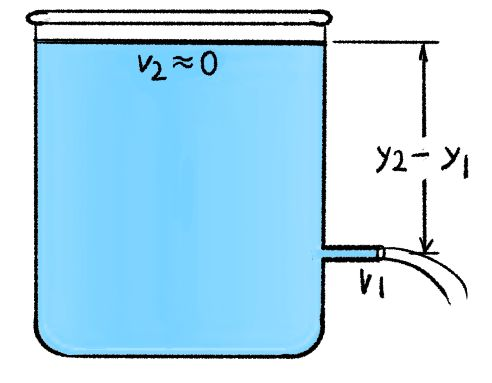
\includegraphics[height=2.in]{images/Bernoulli2.jpg}
    \caption{Exercise \theexample }
    \label{0}
  \end{center}
\end{figure}

where $h = y_2 - y_1$, and $A_1$ and $A_2$ are the areas of the
opening and of the top surface, respectively. Assume $A_1 << A_2$
so that the flow remains
nearly steady and laminar.
% Second Section %%%%%%%%%%%%%%%%%%%%%%%%%%%%%%%%%%%%%%%%%%%%

% \stepcounter{example}
% \section*{Exercise \theexample \footnote{12.93 from Sears and Zemansky}}


% Two very large open tanks $A$ and $F$ contain
% the same liquid. A horizontal pipe BCD, having a constriction at C
% and open to the air at D, leads out of the bottom of tank A, and a
% vertical pipe E opens into the constriction at C and dips into the
% liquid in tank F. Assume streamline flow and no viscosity. If the
% cross-sectional area at C is one-half the area at D and if D is a distance $h_1$
% below the level of the liquid in A, to what height $h_2$ will
% liquid rise in pipe E? Express your answer in terms of h1.

% \begin{figure}[h!]
%     \begin{center}
%       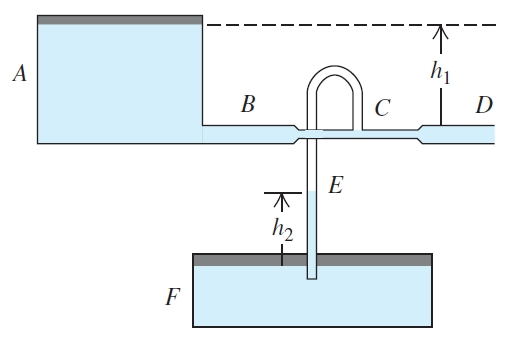
\includegraphics[height=2.4in]{images/1.jpg}
%       \caption{Exercise \theexample }
%       \label{1}
%     \end{center}
%   \end{figure}

% Third Section %%%%%%%%%%%%%%%%%%%%%%%%%%%%%%%%%%%%%%%%%%%%

\stepcounter{example}
\section*{Exercise \theexample \footnote{12.94 from Sears and Zemansky}}

The horizontal pipe
shown in Fig. \ref{2} has
a cross-sectional area of
$40~cm^2$at the wider portions
and $10~cm^2$ at the constriction.
Water is flowing in the
pipe, and the discharge from
the pipe is $6\times10^{-3}~m^3/s$
Find (a) the flow
speeds at the wide and the narrow
portions; (b) the pressure difference between these portions;
(c) the difference in height between the mercury columns in the
U-shaped tube.



\begin{figure}[h!]
    \begin{center}
      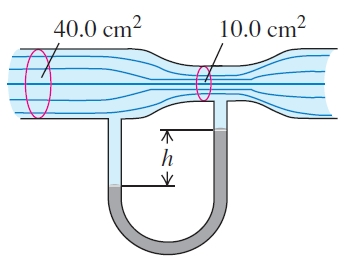
\includegraphics[height=2.4in]{images/2.jpg}
      \caption{Exercise \theexample }
      \label{2}
    \end{center}
  \end{figure}


% % Fourth Section %%%%%%%%%%%%%%%%%%%%%%%%%%%%%%%%%%%%%%%%%%%%

  \stepcounter{example}
  \section*{Exercise \theexample  \footnote{12.95 from Sears and Zemansky} }

  A liquid flowing from a vertical pipe has a definite shape
  as it flows from the pipe. To get the equation for this shape, assume
  that the liquid is in free fall once it leaves the pipe. Just as it leaves
  the pipe, the liquid has speed $v_0$ and the radius of the stream of liquid
  is $r_0$ (a) Find an equation for the speed of the liquid as a function
  of the distance y it has fallen. Combining this with the
  equation of continuity, find an expression for the radius of the
  stream as a function of y. (b) If water flows out of a vertical pipe at
  a speed of $1.2~m/s$ how far below the outlet will the radius be
  one-half the original radius of the stream?


% % Fourth Section %%%%%%%%%%%%%%%%%%%%%%%%%%%%%%%%%%%%%%%%%%%%

\stepcounter{example}
\vspace{20 mm}
\section*{Exercise \theexample  }
Let us make a toy model of a fluid with Octave.

\begin{figure}[h!]
  \begin{center}
    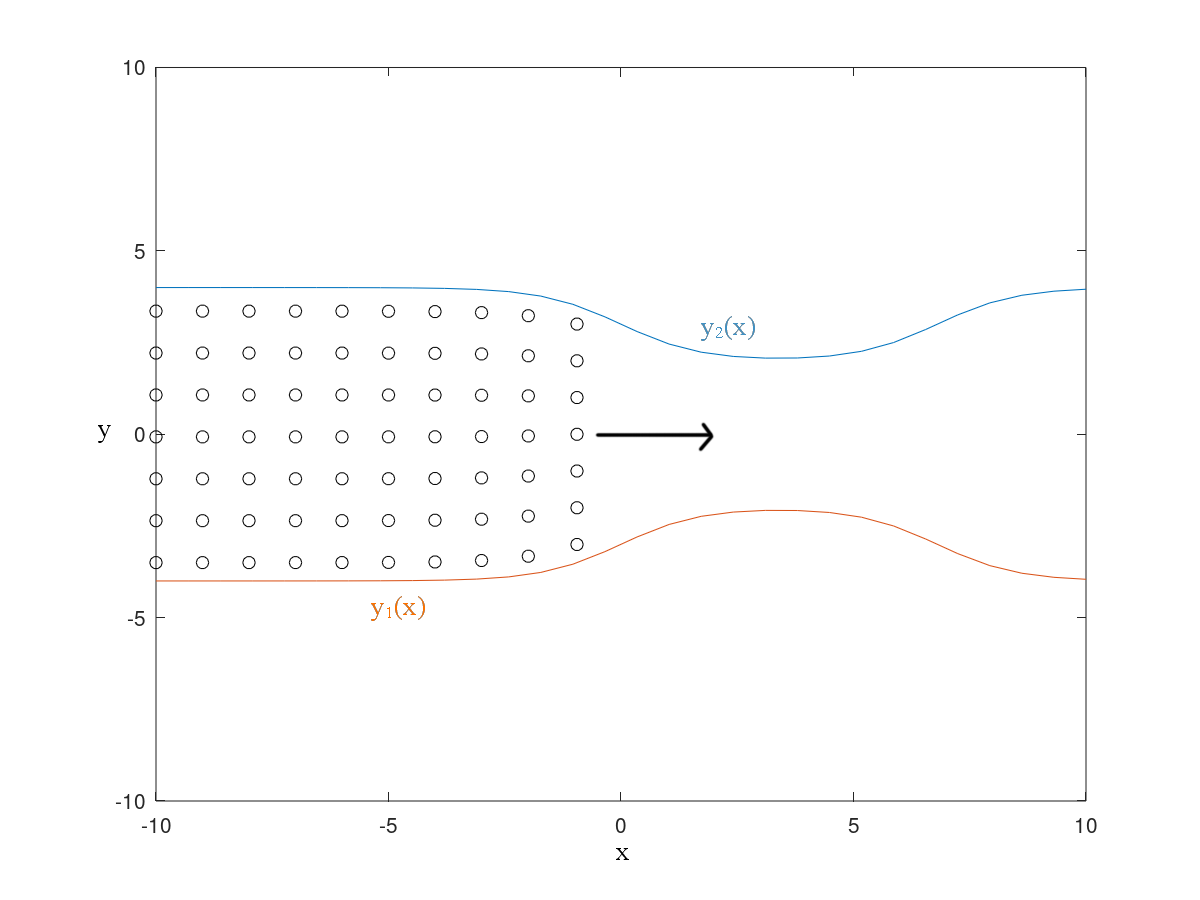
\includegraphics[height=3.6in]{images/fluid_sim.png}
    \caption{Toy model of a fluid. }
    \label{2}
  \end{center}
\end{figure}



\begin{itemize}
  \item The walls of the tube are defined by the functions: 

\end{itemize}


\begin{eqnarray*}
  Y_1(x)&=&-tanh(Ax)+tanh(Ax-B)+B~  (A=0.06,~B=4)\\
  Y_2(x)&=&-Y_1(x)\\
\end{eqnarray*}



\begin{itemize}

  \item Create a mesh grid in the plane (x,y).
  \item Create a matrix containing the particles positions.
  \item The velocity at the point $(0,0)$ is $\vec{v}_0=(0.5,0)$.
  \item Create a velocity vectorial field: assign a velocity to each point in the mesh. The $y$ component of the velocity is always $0$.
  \item \textbf{Start time step}
  \item For each time step actualize the particles positions: each particle is going 
  to get a velocity according to its position (use the function interp2). 
  \item The $y$ component of the particles must satisfy: $y_1<y<y_2$
  \item Make a plot for each time step and build an animation.
\end{itemize}




\end{document}


